\documentclass[a4paper,11pt]{report}
\usepackage[T1]{fontenc}
\usepackage[utf8]{inputenc}
\usepackage{lmodern}
\usepackage[english]{babel}
\usepackage{amsfonts}
\usepackage{hyperref}
\usepackage{graphicx}
\usepackage{subcaption}
\usepackage{float}

\title{Technical report from 31/01/2014 to 26/07/2014}
\author{Rafael Reggiani Manzo}

\begin{document}

\maketitle
\tableofcontents

\chapter{Previous meeting}
  \section{What was presented}
  Last time we met I've showed you my tentative on uncertainty regions segmentation for the whole \textit{corpus callosum} which produced no results despite the various forms of clustering that I tried to employ using FA, MD, TC, TV and RD values.

  \section{Next steps}
  So you've suggested to me to separate a regions where we can say for sure that there is uncertainty, for example where the fibre tracking have a curvature of 60 degrees, so we can be sure if I'm segmenting something useful or not.

\chapter{Work done}
So I separated a region of interest from the fibre tracking starting at the \textit{corpus callosum}.

, produced the FA map for this region, discretized it's values so I could finally apply the segmentation algorithm.

\section{Selecting the region of interest}
  First was applied the fibre tracking (adaptative Rung-Kutta 4) to the corpus callosum. But, instead of stopping the fibre when it has a curvature larger then 45 degrees, it was stopped for 60 degrees, producing the following image \ref{fig:fibres}.

  \begin{figure}[H]
    \includegraphics[width=1\linewidth]{imgs/cc-expanded-fibers.png}
    \caption{3D view of \textit{corpus callosum} with fibers tracked by the adaptive Runge-Kutta algorithm on Bio Image Suite.}
    \label{fig:fibres}
  \end{figure}

  And then exported these fibres as mask (\ref{fig:fibres-mask})

  \begin{figure}[H]
    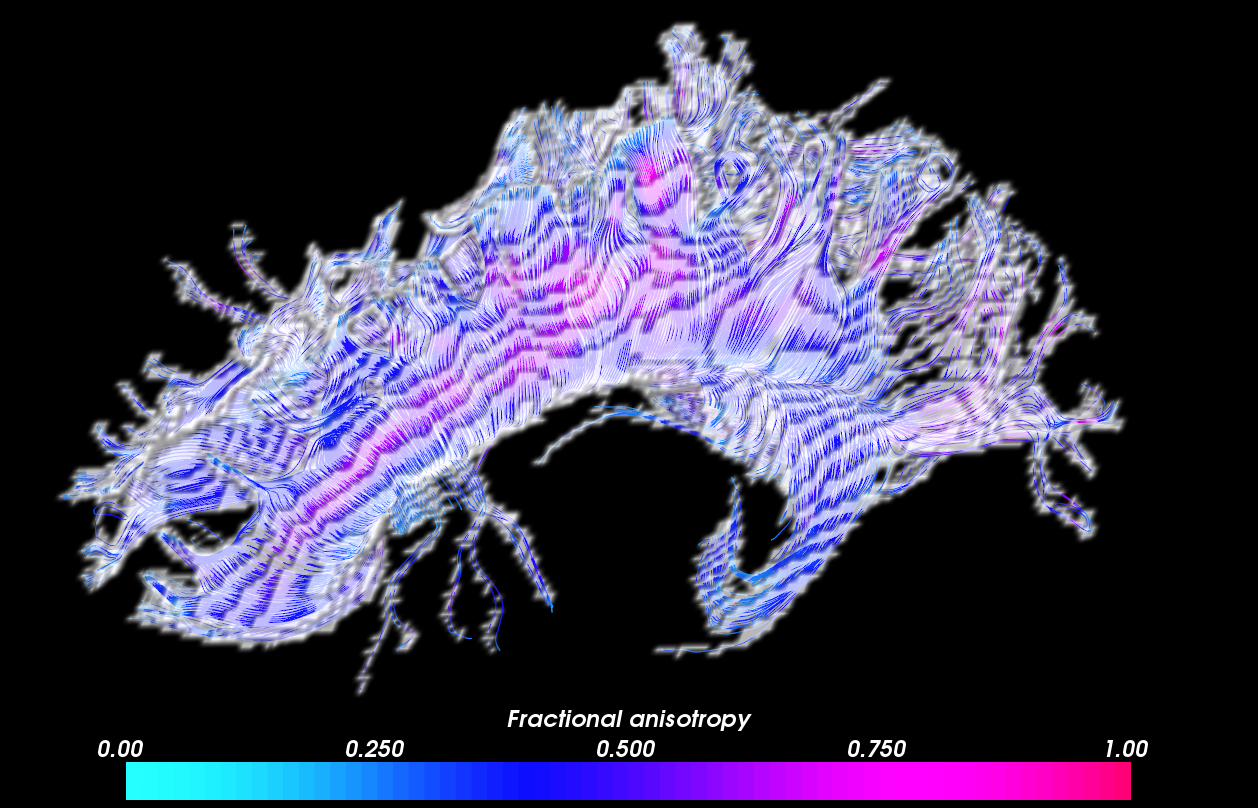
\includegraphics[width=1\linewidth]{imgs/cc-expanded-fibers-mask.png}
    \caption{3D view of \textit{corpus callosum} with fibres tracked by the adaptive Runge-Kutta algorithm on Bio Image Suite combined with the exported mask.}
    \label{fig:fibres-mask}
  \end{figure}

  Finally cropped the mask at region where the fibre curvature is anatomically impossible (the coordinates $i$ from 83 to 96, $j$ from 65 to 88 and $k$ from 33 to 49).

  \begin{figure}[H]
    \includegraphics[width=1\linewidth]{imgs/cc-expanded-fibers-mask-croped.png}
    \caption{3D view of \textit{corpus callosum} with fibres tracked by the adaptive Runge-Kutta algorithm on Bio Image Suite combined with the exported mask cropped at region of interest.}
    \label{fig:fibres-mask-croped}
  \end{figure}

  \section{Applying a classical clustering algorithm}
  As mentioned before the algorithm applied in order to create the voxel clusters was DBSCAN\footnote{Ester, Martin, et al. ``A density-based algorithm for discovering clusters in large spatial databases with noise.'' Kdd. Vol. 96. 1996.}. It is based on similarity between items in order to group them into clusters. That's why it was my first choice.

  But, unfortunately, it takes three parameters to run and I wasn't able to find out which parameters combined together would cluster for me just the uncertainty region. The results with this kind of algorithm were always lots of grouped voxels that had no visual meaning.

  If in the future I decide to get back to this algorithm probably I'll have to write some kind of previous training in order to figure out the parameter that approximate the best the uncertainty region as one cluster.

  \section{Applying a classical image segmentation algorithm}
  After giving up with the clustering algorithms for now, inspired by a class that I took last semester, I noticed that actually my problem could be understood as one of image segmentation: one wants to segment the uncertainty regions from the certainty regions.

  Then I decided to use the watersheds algorithm\footnote{Vincent, Luc, and Pierre Soille. ``Watersheds in digital spaces: an efficient algorithm based on immersion simulations.'' IEEE transactions on pattern analysis and machine intelligence 13.6 (1991): 583-598.}. Briefly, it is based on the idea of understanding a greyscale image as series of elevations and then trying to figure out where would a water drop stop if it is dropped at each point of the image. So finally, the points of the image which leads to the same locations are grouped together.

  For my purpose I've adopted the discretized FA map (given a FA map, for each voxel multiply it by 100 and then take it's floor) of the region of interest as my greyscale image. Then after applying the algorithm I've got the following:

  \begin{figure}[H]
    \includegraphics[width=1\linewidth]{imgs/cc-expanded-fibers-mask-croped-watersheds.png}
    \caption{3D view of \textit{corpus callosum} with fibres tracked by the adaptive Runge-Kutta algorithm on Bio Image Suite combined with the exported mask cropped at region of interest and then segmented.}
    \label{fig:fibres-mask-croped-segmented}
  \end{figure}

  For a better comparison, we can see side by side the zoomed regions for the original region and the segmentation result:

  \begin{figure}[H]
    \centering
    \begin{subfigure}[t]{.49\textwidth}
      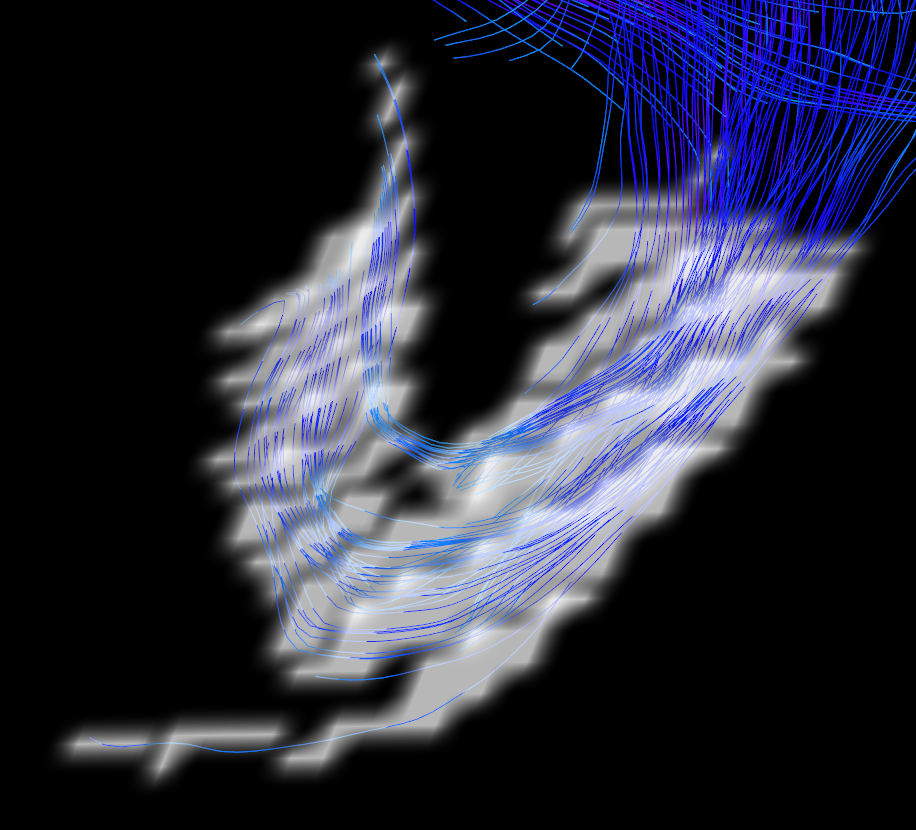
\includegraphics[width=1\linewidth]{imgs/cc-expanded-fibers-mask-croped-zoomed.png}
      \caption{Interest region zoom}
      \label{subfig:fibres-mask-croped-zoomed}
    \end{subfigure}\hfill%
    \begin{subfigure}[t]{.49\textwidth}
      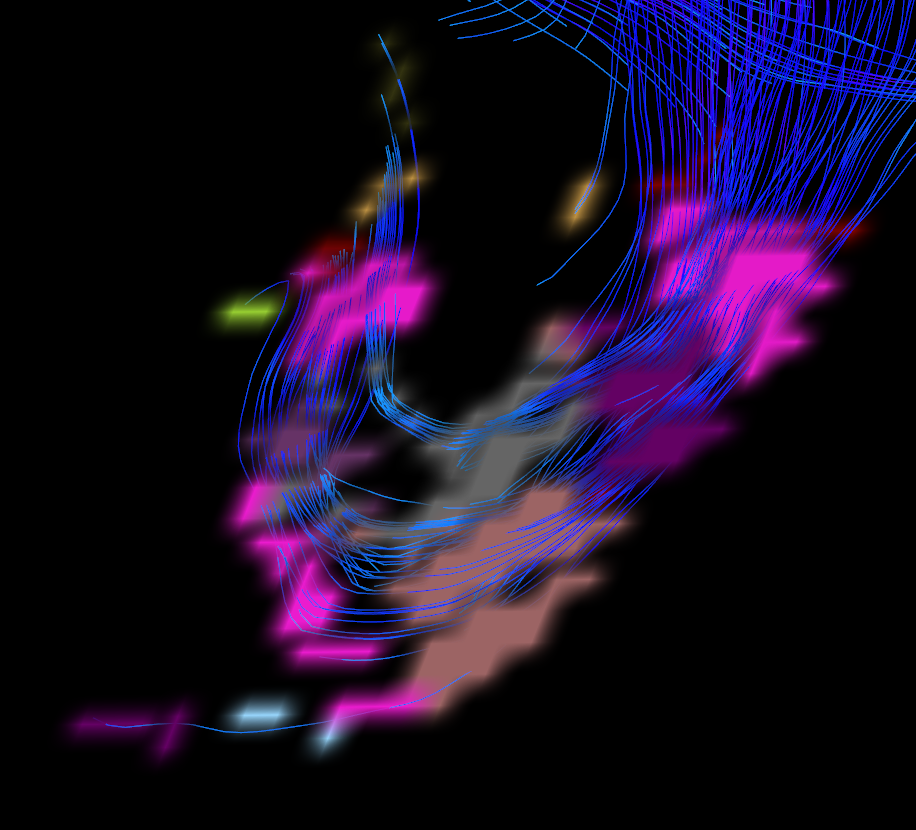
\includegraphics[width=1\linewidth]{imgs/cc-expanded-fibers-mask-croped-watersheds-zoomed.png}
      \caption{Interest region segmented zoom}
      \label{subfig:fibres-mask-croped-segmented-zoomed}
    \end{subfigure}\hfill
  \end{figure}

  It is possible to notice that the grey region from the segmentation is the which better approximates the uncertainty region at the corner that the fibre do.

  \begin{figure}[H]
    \centering
    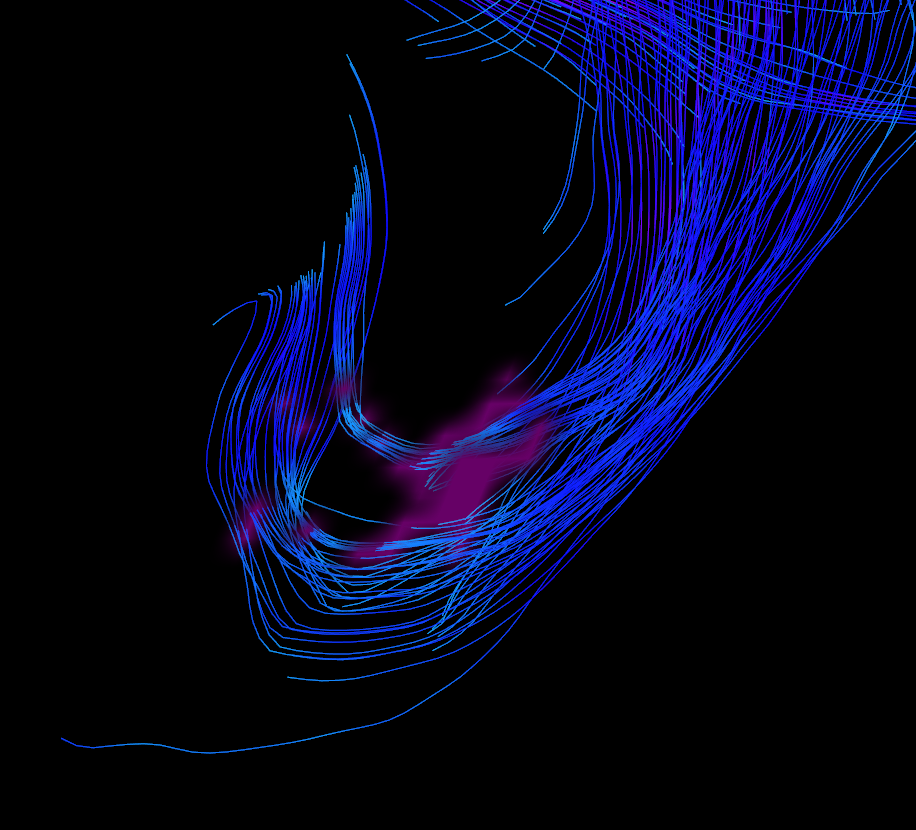
\includegraphics[width=0.6\linewidth]{imgs/cc-expanded-fibers-mask-croped-watersheds-region7-zoomed.png}
    \caption{Isolated segmented region zoom.}
    \label{fig:fibres-mask-croped-segmented-region}
  \end{figure}

\chapter{Next steps}
I hope I'm right to say that this image segmentation algorithm presented last finally was able to find an uncertainty region. If so, the next steps would be to map a lot more interest regions and then try to apply the same process to them.

If successful for the new interest regions, try to compare the segmented uncertainty regions in order to find a similarity between them so the process of find the segmented uncertainty region among all the other segmented can get automated by this criteria.
\end{document}